\def\year{2017}\relax
%File: formatting-instruction.tex
\documentclass[letterpaper]{article}

\usepackage{graphicx}
\usepackage{amsmath}
\usepackage{amssymb}
\usepackage{amsthm,mathrsfs,amsfonts,dsfont}
\usepackage{algorithm}
\usepackage{algorithmic}
\usepackage{threeparttable}
\usepackage{multirow}
\usepackage{subfigure}
\usepackage{color}
\usepackage{epstopdf}
\usepackage{bm}
%\usepackage[vlined,boxed,ruled]{algorithm2e}
\usepackage{url}
\usepackage{xspace}

\newtheorem{corollary}{Corollary}
\newtheorem{definition}{Definition}
\newtheorem{theorem}{Theorem}
\newtheorem{proposition}{Proposition}
\newtheorem{lemma}{Lemma}
\newtheorem{remark}{Remark}



\usepackage{aaai17}
\usepackage{times}
\usepackage{helvet}
\usepackage{courier}



\def\grad{\mbox{\text{\textbf{grad}}}}
\def\bzero{{\bf{0}}}

\def\bD{{\bf D}}
\def\bI{{\bf I}}
\def\bE{{\bf E}}
\def\blambda{{\bm \lambda}}
\def\calL{{\mathcal{L}}}
\def\calC{{\mathcal{C}}}
\def\calS{{\mathcal{S}}}
\def\calF{{\mathcal{F}}}
\def\bL{{\bf L}}
\def\bO{{\bf O}}
\def\bU{{\bf U}}
\def\bV{{\bf V}}
\def\dsR{\mathds{R}}
\def\bX{{\bf X}}
\def\bx{{\bf x}}
\def\btx{{\tilde{\bf x}}}
\def\by{{\bf y}}
\def\bw{{\bf w}}
\def\btw{{\tilde{\bf w}}}
\def\tK{\tilde{K}}
\def\txi{\tilde{\xi}}
\def\tildeb{{\tilde{b}}}
\def\tphi{{\tilde{\phi}}}
\def\bz{{\bf z}}
\def\br{{\bf r}}
\def\bv{{\bf v}}
\def\bb{{\bf b}}
\def\bp{{\bf p}}
\def\bA{{\bf A}}
\def\bI{{\bf I}}

\def\bx{{\bf x}}
\def\bX{{\bf X}}
\def\by{{\bf y}}
\def\bY{{\bf Y}}
\def\bw{{\bf w}}
\def\bW{{\bf W}}
\def\balpha{{\bm \alpha}}
\def\bmu{{\bm \mu}}
\def\bK{{\bf K}}
\def\bg{{\bf g}}
\def\bp{{\bf p}}
\def\p{p}
\def\bP{{\bf P}}

\def\balpha{{\bm \alpha}}
\def\bbeta{{\bm \beta}}
\def\eg{{\emph{e.g.}}}
\def\zerocolumn{{\bf 0}}

\def\ttTP{{\tt TP}}
\def\ttFP{{\tt FP}}
\def\ttFN{{\tt FN}}

\def\st{{\text{s.t.}}}
\def\rank{{\text{rank}}}
\def\Tr{{\text{Tr}}}

\def\yanred{\textcolor{red}}
\def\yanblue{\textcolor{blue}}


\frenchspacing
\setlength{\pdfpagewidth}{8.5in}
\setlength{\pdfpageheight}{11in}
\pdfinfo{
/Title (Insert Your Title Here)
/Author (Put All Your Authors Here, Separated by Commas)}
\setcounter{secnumdepth}{0}
 \begin{document}


% The file aaai.sty is the style file for AAAI Press
% proceedings, working notes, and technical reports.
%



\title{Robust Late Fusion Based on Matrix Factorization}

%\author{AAAI Press\\
%Association for the Advancement of Artificial Intelligence\\
%2275 East Bayshore Road, Suite 160\\
%Palo Alto, California 94303\\
%}

\maketitle



\begin{abstract}
% First: A big picture of the scenario which we would consider
In many real world applications, data can be represented in multiple ways/features, which would describe various characteristics of data.
Many works have shown that it could often improve the performance to make use of these features together.
% Second: what BIG problem would we like to solve?
Late fusion, which combines the predictions of multiple features, is a commonly used approach to generate the final decision for a test instance.
% Third: specify the detailed problem: find a precise position for our paper
However, it is ubiquitous that different features would dispute on some data, leading to the requirement of outlier rejection for late fusion algorithms.
% Fourth: general introduction of our method
In this paper, we propose an efficient matrix factorization based approach to fuse predictions from multiple sources, which could
relieve the performance degeneration caused by the controversy of multiple features on test data.
% Some unvalued sentence(s)
Extensive experiments demonstrate that the proposed method is effective to remove outliers and improve fusion performance.

\end{abstract}




\section{Introduction}


%背景 多model融合
Feature extraction, which transforms raw data into numerical features, is a prerequisite for most real world applications.
There are often multiple ways to generate numerical features from raw data.
For example, for image data, one can extract hand-crafted features such as scale-invariant feature transform
(SIFT)~\cite{loweijcv2004distinctive}, Histograms of Gradients (HOG)~\cite{dalalcvpr2005histograms} and trained convolutional neural networks (CNNs) features~\cite{krizhevskynips2012imagenet}.
Text data can be represented by term frequency–inverse document frequency (tf-idf)~\cite{manning2008introduction} and word2vec~\cite{mikoloviclr2013efficient}.
%Videos can be represented by Dense Trajectories~\cite{Wang2011Action}, CNNs~\cite{xucvpr2015discriminative}, \etc.
%\cite{szegedy2015going,chatfield2014return,he2015deep,simonyan2014two,xucvpr2015discriminative}
Each category of features tends to capture a specific characteristics of data.
A model trained on an individual feature could be biased and hence obtains an unsatisfactory performance.
Existing works have investigate the performance improvement by combining multiple features in real world applications~\cite{gehler2009feature,ye2012robust,xuiccv2013feature,lai2015learning}.


%背景 多model融合
%Image or video data in the real world can be represented in multiple features.
%For example, motion features of videos can be extracted by Dense Trajectories~\cite{Wang2011Action}.
%Shape features of frames can be represented by Histograms of Oriented Gradients~\cite{dalal2005histograms} and 
%Scale-Invariant Feature Transform~\cite{lowe2004distinctive}, and some complex CNN features for both frames and 
%sequences can be trained by ~\cite{szegedy2015going,chatfield2014return,he2015deep,simonyan2014two,Xu_2015_CVPR}.
%Each feature contains rich information of real data, which can not capture all views of our data.
%A single classifier model will bias on some characteristics of training data based on different features.
%It can significantly improve the performance by combining multiple features together and capturing more views on data.



%% late fusion is a common sigle model -> single feature, 介绍late fusion
Late fusion, a typical approach to obtaining the final decision on testing data, aims to fuse the predictions from each individual feature.
A commonly used method is to learn weights for predictions of each feature and linearly combine them, which has a number of variations~\cite{gehler2009feature,xuiccv2013feature,lai2015learning}.
Among these algorithms, multiple kernel learning (MKL)~\cite{lanckriet2004learning,Rakotomamonjy2008Simplemkl} is often used to train such a weighted combination.
However, a single feature may produce corrupted predictions on some data, which likely degenerates performance.
To deal with this issue, therefore, some works formulate it as a robust low rank matrix recovery problem~\cite{gaoijcai2016robust,ye2012robust} by nuclear norm minimization.
Nevertheless, nuclear norm minimization applied in these works requires singular value decompositions (SVDs), which would be computationally unaffordable for large matrices.


%% late fusion is a common sigle model -> single feature, 介绍late fusion
%%Late fusion is a common method to make the combination of different features. Single model is firstly trained on different features using Support Vector Machine(SVM) or other classifiers, and then late fusion methods combine the predicted decision results of each single model to decide the final result.
%% A popular family of late fusion algorithm is that estimate a learned weight for each single model and then fuse the weighted prediction results by simple summation. Multiple Kernel Learning(MKL)~\cite{lanckriet2004learning,Rakotomamonjy2008Simplemkl} based method learn a linear combination to fuse multiple predicted scores, many works optimize the MKL based late fusion method by leading thresholding, specific weights or robust constraint into algorithm, such as \cite{gehler2009feature,xuiccv2013feature,lai2015learning}.
%% \yanred{The alogrithms proposed in Robust Principal Components Analysis(RPCA) might also be used for late fusion, which are capable to find the anomalous results among multiple classifers~\cite{gaoijcai2016robust}. }
%%这提了Gao,下一段也提了Gao这样好么?

%%In the early fusion, a linear combination or more complex functions,eg. 3D convolution , of different features is utilized to capture inner correlation bettwen each model, such as \cite{Feichtenhofer2016Convolutional}. A more simple but effective method in early fusion is to calculate multiple kernel matrix from different features and then average them together to train a SVM classifier.Another fusion technique is late fusion, which train classifiers of seperate features and then fuses the results based on the predicted scores, such as \cite{gehler2009feature} learns a linear combination on decision values of individual features to boost the performance of single model.
%%Most previous works in late fusion focus on how to learn weights on different models, (disadvantage?)


%% 不同的features 会有意见不同的时候,具体 outlier rejection,might [Gao low rank sparse loss, but the nuclear norm
%% scale poorly , expensive single vd(SVDs) present of , the other way of low MF foucs on least square smooth function
%% least square loss is sensitive to outlier
%% it's unclear to extend MF to nonsmooth function .
%% In this paper we proposed a
%%Another issue in late fusion is that some works based on MKL \cite{xuiccv2013feature} poor ability to extend their algorithm to large scale data, the ensemble clustering alogrithm \cite{gaoijcai2016robust}, which could alse used in fusion, use a matrix inversion learding into a high time complexity.
%% It is ubiquitous that multiple classifers based on different features would have disagreements on some data, which motivates the outlier rejection might solve this problem. There are some researchers have ability to reject the outlier of multiple results, such as \cite{gaoijcai2016robust} use low rank sparse $\ell_{1,2}$ loss and nuclear norm to solve, which are poorly to extend to large scale data due to the expensive cost of Singular Value Decomposition(SVDs) present in the alogrithm. The other research on matrix factorization foucs on least square smooth loss funcion, which is sensitive to outlier and it's unclear to extend matrix factorization to nonsmooth $\ell_{1,2}$ loss.




To prevent from the expensive nuclear norm minimization, in this paper, we propose a more efficient matrix factorization algorithm to recover the underlying low rank label matrix.
As for outlier detection, as shown in Figure~\ref{fig:framework}, we apply robust $\ell_{1,2}$ loss to remove the outlier columns in the label matrix.
Most existing matrix factorization optimization methods, however, only consider smooth loss functions, rather than the nonsmooth loss.
We thus in particular present an approach based on augmented Lagrangian multiplier (ALM) to extend matrix factorization methods to nonsmooth problems.
The main contributions are summarized as below:
\begin{itemize}
  \item We propose an efficient late fusion algorithm based on matrix factorization.
  \item We extend existing matrix factorization algorithms from smooth least square loss to nonsmooth $\ell_{1,2}$ loss.
  \item Empirical studies show significantly improvement of our proposed method compared to existing late fusion algorithms.
\end{itemize}

%%In this paper, we introduce an efficient matrix factorization based alogrithm for late fuse, named Outlier Rejection for Late Fusion(ORLF).
%%We utilize the robust $\ell_{1,2}$ nonsmooth objective fuction~(\ref{eq:typical_mc}) to remove the outlier results among different classifiers. We introduce the low rank constraint to maintain the consistency among differernt classifers.
%%The formulation can be written as below:

%\begin{align}\label{eq:typical_mc}
%  \min_{\bX} ~&~ || \bX - \bL ||_{1,2}   \nonumber \\
%  \st        ~&~ \rank(\bX) \leq k  ,
%\end{align}
%\noindent

%L a is observed matrix, represent the label indicator matrix in our vision recoginition case. X is a low rank matrix recovered from L. Rank function measures the rank of a matrix. $|| \bX ||_{1,2} = \sum_{j = 1}^{M} \sqrt{\sum_{i=1}^{N} \bX_{ij}} = \sum_{j=1}^{M} || \bX_{.j} ||_2$, where $\bX \in \dsR^{N \times M}$.
%Problem~(\ref{eq:typical_mc}) is NP-hard due to the presence of the low rank constraint. For the sake of efficiency on large scale matrices, we consider matrix factorization approaches to optimize it, which can be written as below:
%\begin{align}\label{eq:mf_l21}
%  \min_{\bX} ~&~ || \bL - \bX ||_{1,2}    \nonumber \\
%  \st        ~&~ \bX = \bU \bV,~\bU \in \dsR^{N \times k},~\bV \in \dsR^{k \times MK} .
%\end{align}
%\noindent
%Most existing matrix factorization optimization methods only consider smooth loss functions, but the $\ell_{1,2}$ loss in \ref{eq:mf_l21} is nonsmooth. In our proposed method(ORLF), we apply augmented Lagrangian multiplier (ALM) to optimize the nonsmooth objective function efficiently.

%Our main contribution can be summarized as below:
%\begin{itemize}
%  \item We propose an efficient late fusion algorithm based on matrix factorization to do outlier rejection.
%  \item We extend matrix factorization alogrithm to handle $\ell_{1,2}$ norm function.
%  \item Out proposed method empirically shows significantly improvement than other late fusion algorithms.
%\end{itemize}

%A single clustering result could be inaccurate, so some researchers study ensemble clustering methods to boost the performance,
%such as the algorithms proposed in~\cite{yiicdm2012robust,gaoijcai2016robust}, to name a few.



\section{Related Work}
%% Matrix factorization
%% Fusion Methods
%%

Matrix factorization has attracted increasing attention recently,
and many manifold optimization based algorithms have been proposed by exploiting the manifold geometry.
Based on manifold optimization, fixed-rank matrices are supposed to belong to a smooth matrix manifold~\cite{Absil2008OAMM,vandereycken2013lowrank}.
In~\cite{vandereycken2013lowrank}, the authors propose a low rank geometric conjugate gradient (LRGeomCG) method.
In~\cite{rtrmc2011boumal}, first- and second-order Riemannian trust-region methods are applied to solve the low rank matrix completion by exploiting the low rank constraint.
In~\cite{Bonnabel2011}, a linear regression algorithm is proposed, where the parameter of this algorithm is a fixed-rank matrix based on the Riemannian manifold geometry.
In~\cite{Mishra2012}, the authors propose a quotient geometric matrix completion method.
The authors in~\cite{grouse2010Balzano} propose an online algorithm for tracking subspaces, Grassmannian rank-one update subspace estimation.
In~\cite{ngonips2012scaled}, a gradient methods based on scaled metric on the Grassmann manifold is proposed.
The authors in~\cite{Wen2012} propose a low-rank matrix fitting algorithm is proposed to solve large scale matrix completion problems by exploiting nonlinear successive over-relaxation.
In~\cite{RechtNIPS2011hogwild}, a lock-free approach to parallelizing stochastic gradient descent is proposed.
However, all these matrix factorization methods only consider the general least square loss, which cannot be directly applied to handle $\ell_{1,2}$ loss.


MKL based method is a simple but efficient way to combine different features for multi-model fusion,
and many improved algorithms have been proposed by introducing more constraint, boosting methods and other optimization.
In~\cite{vedaldi2009multiple}, the authors use MKL to learn an optimal combination of exponential ${\chi}^2$ kernels capturing a different feature channel. 
In~\cite{gehler2009feature}, boosting approaches are proposed to ensemble different features, which learns the correct weighting of multiple predicted confidence scores from different models.
In~\cite{natarajan2012multimodal}, the authors propose a two-step strategy employing MKL and late score fusion methods to combine diverse features, specifically on event detection tasks.
In~\cite{lai2015learning}, a sample specific late fusion based on graph Laplacian with RankSVM style constraints is proposed,
which learns sample specific fusion weights by diffusing the information from labeled samples to the unlabeled one.
In~\cite{xuiccv2013feature}, a optimization algorithm are proposed to combine diverse decision values, 
which learns the weights, thresholding and smoothing parameters in a joint framework.
However, all these mkl based fusion methods or others only learn weights to combine different basic models, which do not consider the outlier rejection in the fusion process specifically.

%% Latent Fusion,

\section{The Proposed Approach}
We first elaborate the formulation of our ORLF algorithm. Then we show the details about how to use augmented Lagrangian multiplier (ALM) to solve the $\ell_{1,2}$ objective function. Finnaly we introduce our post process strategy to convert the recovered matrix X in \ref{eq:mf_l21} to the final predicted label.


\subsection{Problem Formulation}
Suppose there are n testing instances, we denote each instance as a variable $x_i{\in}\dsR^{d}(1{\leq}i{\leq}n)$. Assuming we have already training m classifiers, $f_1(x), f_2(x), ... f_m(x)$, per classifier will predict a score vector $s_{ij}, 1{\leq}i{\leq}n, 1{\leq}j{\leq}m $,represent the result of j-th classifier on i-th testing instance. Our goal is to fusion these predicted confidence score vectors. Firstly, we transfer these score vectors to a label matrix P, each colums represent the highest value position of each instance. Then using label assigment, we convert multiple P matrixs into a 01 indicator matrix L, see as{\ref{fig:framework}}.
The core of our proposed algorithm is to apply $\ell_{1,2}$ to capture the outliers as well as anomalous columns in matrix L, and apply a matrix factorization based approach to optimize the objective function as shown below: 

\begin{align}\label{eq:mf_l21}
    \min_{\bX} ~&~ || \bL - \bX ||_{1,2}    \nonumber \\
    \st        ~&~ \bX = \bU \bV,~\bU \in \dsR^{N \times k},~\bV \in \dsR^{k \times MK} .
\end{align}
The k of the low rank constraint in (\ref{eq:mf_l21}) is the number of class in recoginition task.

\begin{figure}[h]
\centering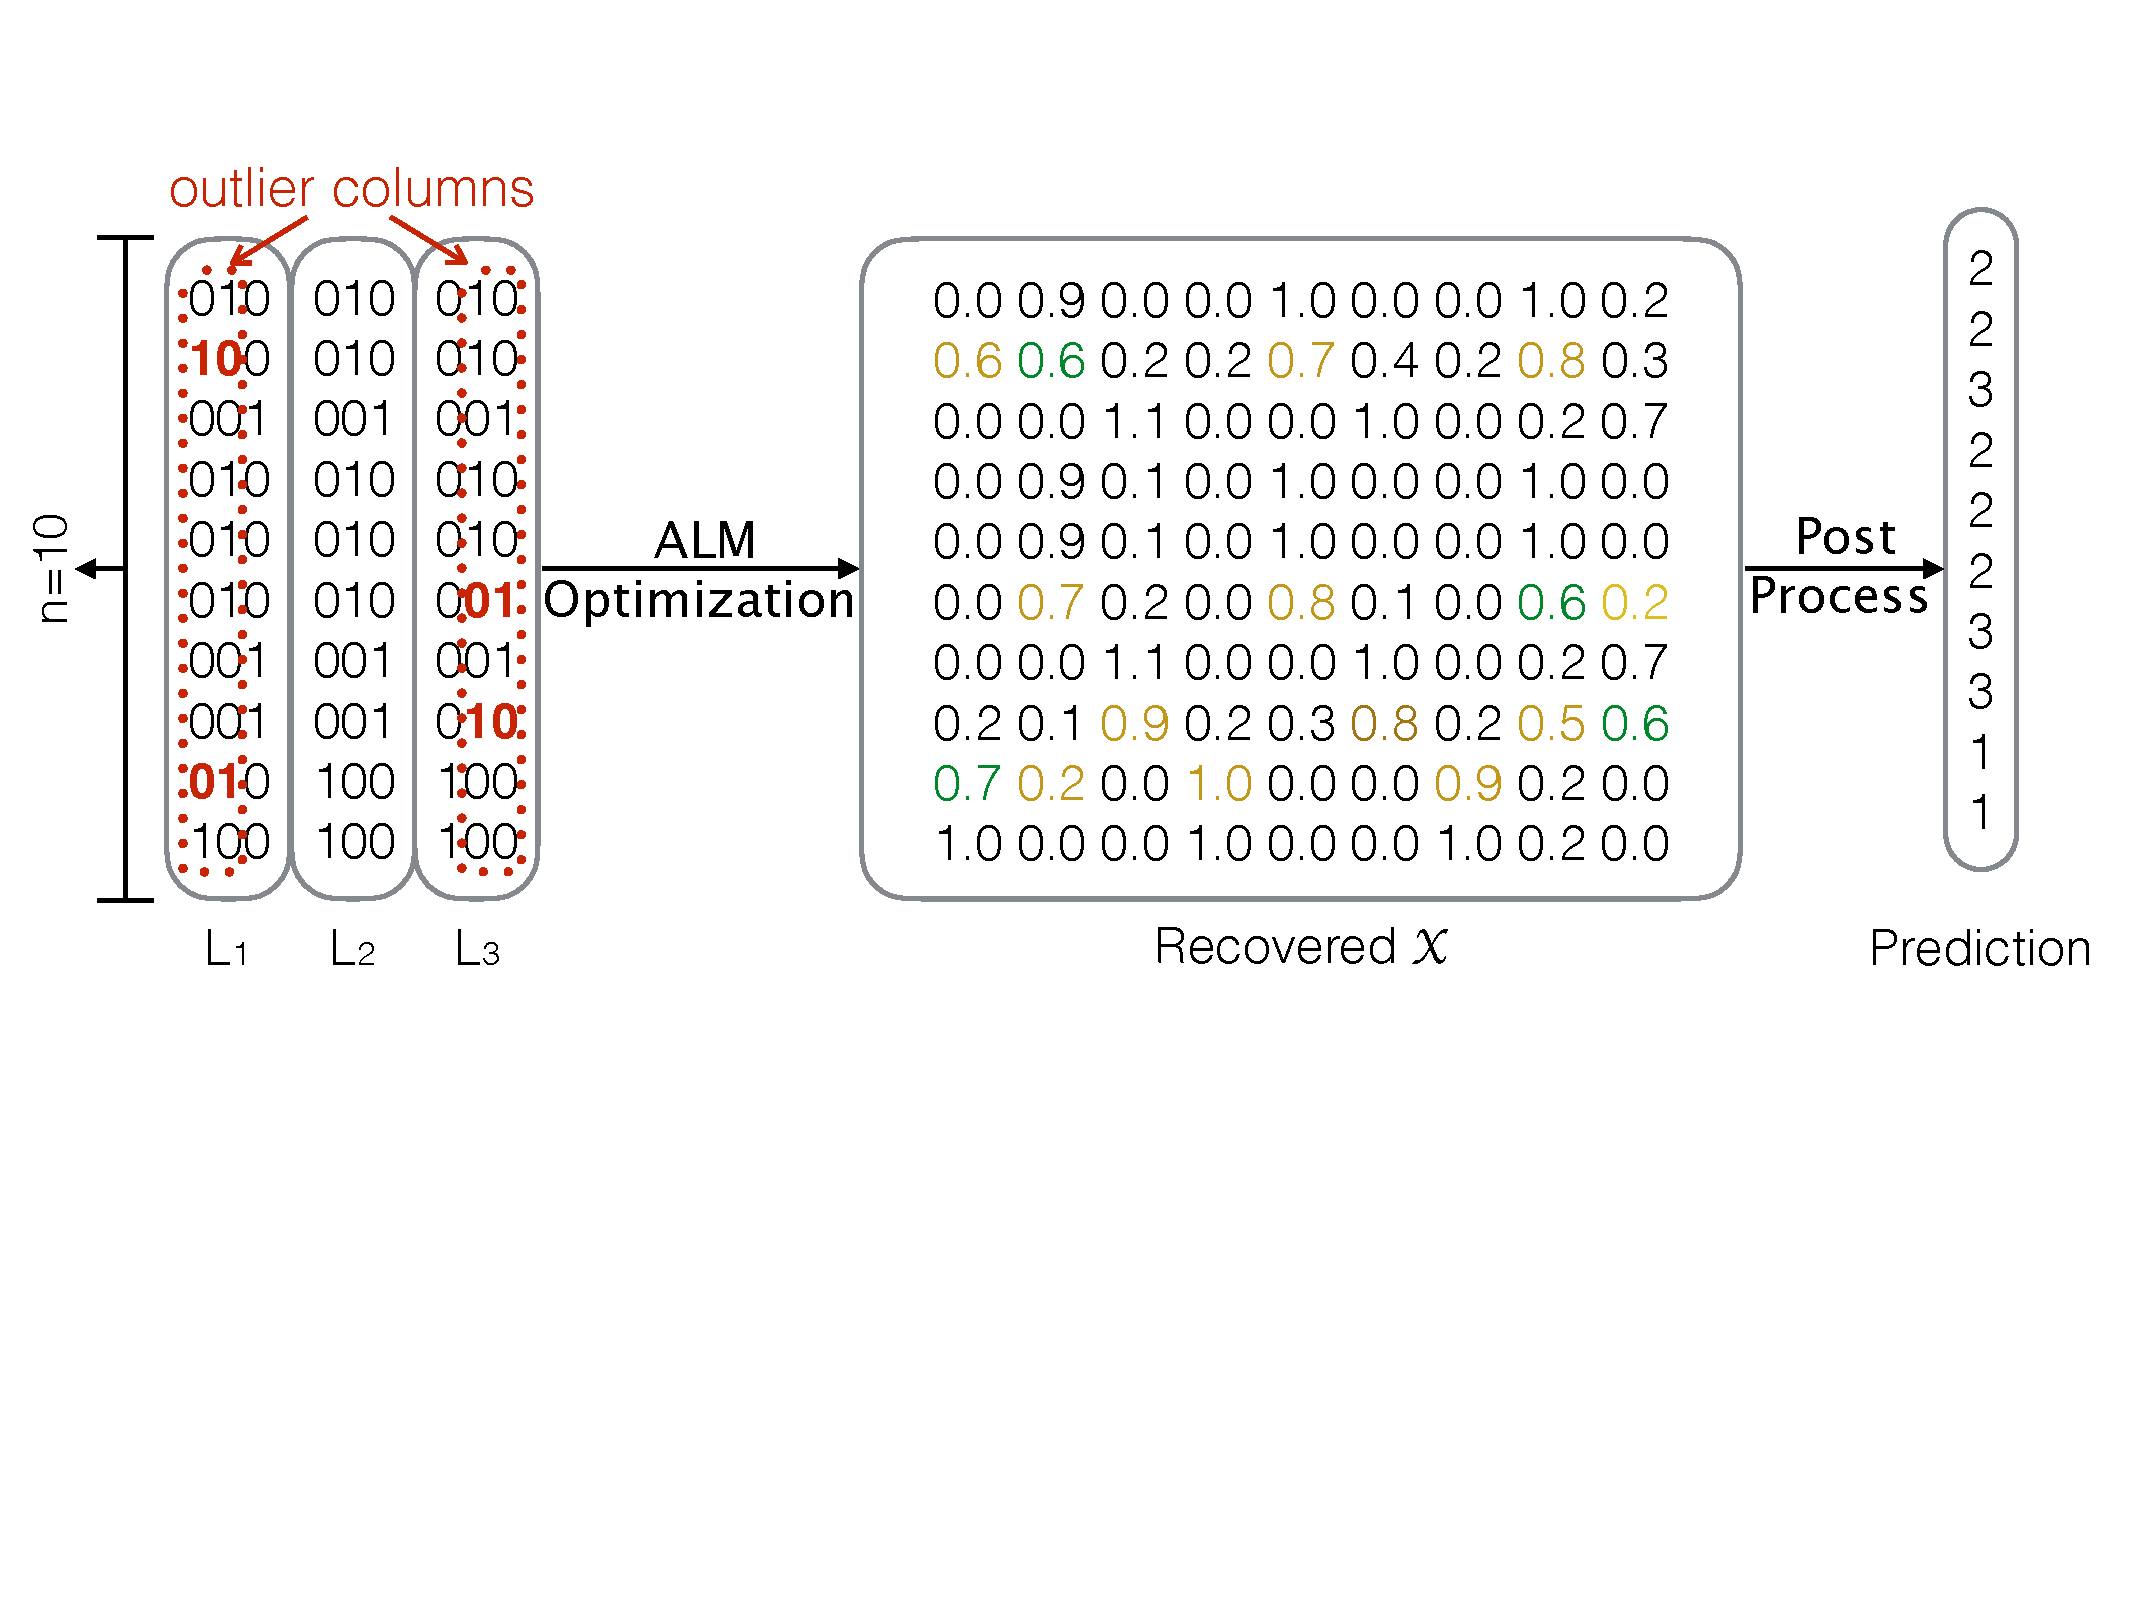
\includegraphics[width=0.45\textwidth]{resource/frame_work.pdf}
\caption{Frame Work}
\label{fig:framework}
\end{figure}


\subsection{ALM Optimization}
Most existing matrix factorization optimization methods only consider smooth loss functions, but the $\ell_{1,2}$ loss in Problem~(\ref{eq:mf_l21}) is nonsmooth.
We apply ALM to optimize the nonsmooth objective function efficiently, desccribed as below:

By introducing a new variable $\bE = \bL - \bX$, we can develop Problem~(\ref{eq:mf_l21}) as below:

\begin{align}\label{eq:mf_l21_constrained}
  \min_{\bE, \bX} ~&~ || \bE ||_{1,2}   \nonumber \\
  \st             ~&~ \bE = \bL - \bX   \nonumber \\
                  ~&~ \bX = \bU \bV,~\bU \in \dsR^{N \times k},~\bV \in \dsR^{k \times MK}
\end{align}
The augmented Lagrangian function of Problem~(\ref{eq:mf_l21}) is as below
\begin{align}\label{eq:lagrangian_l21}
  \calL = & || \bE ||_{1,2} + \langle \blambda, \bL - \bX - \bE \rangle + \frac{\mu}{2} || \bL - \bX - \bE ||_F^2
\end{align}
\noindent
where $\bX = \bU \bV$,
and $\blambda \in \dsR^{MK \times N}$ are the Lagrangian multipliers (or dual variables).
Then we could update $\bX$ and $\bE$ alternatively.


Specifically, to update $\bX$, we consider the following problem:
\begin{align}\label{eq:problem_X}
  \min_{\bX} ~&~ \langle \blambda, \bL - \bX - \bE \rangle + \frac{\mu}{2} || \bL - \bX - \bE ||_F^2  \nonumber  \\
  \st        ~&~ \bX = \bU \bV,~\bU \in \dsR^{N \times k},~\bV \in \dsR^{k \times MK}   .
\end{align}
Problem~(\ref{eq:problem_X}) includes a smooth loss function w.r.t. $\bX$, thus can be solved by a standard matrix factorization method, such as~\cite{yanijcai2015scalable,tanicml2014riemannian,vandereyckensiamjo2013low}.


Problem~(\ref{eq:problem_X}) can also be rewritten as below
\begin{align}\label{eq:problem_X2}
  \min_{\bX} ~&~ \frac{\mu}{2} \Big( || \bL - \bX - \bE ||_F^2 + \frac{2}{\mu} \langle \blambda, \bL - \bX - \bE \rangle + \frac{|| \blambda ||_F^2}{\mu^2} \Big)    \nonumber   \\
             ~&~ - \frac{\mu}{2} \frac{|| \blambda ||_F^2}{\mu^2}   \nonumber \\
  \st.       ~&~ \bX = \bU \bV,~\bU \in \dsR^{N \times k},~\bV \in \dsR^{k \times MK}   .
\end{align}
\noindent
We can obtain the final problem w.r.t. $\bX$:
\begin{align}\label{eq:problem_X3}
  \min_{\bX} ~&~ || \bL - \bX - \bE + \frac{\blambda}{\mu} ||_F^2   \nonumber \\
  \st        ~&~ \bX = \bU \bV,~\bU \in \dsR^{N \times k},~\bV \in \dsR^{k \times MK}   .
\end{align}
\noindent
There are a number of optimization algorithms for Problem~(\ref{eq:problem_X3}), such as LRGeomCG\footnote{\yanred{Code available at~\url{http://www.unige.ch/math/vandereycken/matrix_completion.html}}}.




To update $\bE$, we consider the following problem:
\begin{align}\label{eq:problem_E}
  \yanred{
  \min_{\bE} ~ || \bE ||_{1,2} + \langle \blambda, \bL - \bX - \bE \rangle + \frac{\mu}{2} || \bL - \bX - \bE ||_F^2   .
  }
\end{align}
\noindent
Similarly, we could reformulate the above problem as below:
\begin{align}\label{eq:problem_E2}
  \min_{\bE} & \frac{2}{\mu} || \bE ||_{1,2} + || \bL - \bX - \bE + \frac{\blambda}{\mu} ||_F^2    .
\end{align}
\noindent
Let $\bY = \bL - \bX + \frac{\blambda}{\mu}$.
The above problem can be efficiently solved by the following column-wise soft-thresholding operator:
\begin{align}\label{eq:column_wise_soft_thresholding}
  \bE_{i} = \calS_{\alpha}(\bY_{i}) = \left\{
    \begin{aligned}
      & \zerocolumn,~\text{if}~ ||\bY_{i}||_2 \leq \alpha   \\
      & \bY_{i} - \frac{\alpha \bY_{i}}{|| \bY_{i} ||_2},~\text{otherwise,}
    \end{aligned}
    \right.
\end{align}
\noindent
where $\bE_{i}$ and $\bY_{i}$ denote the $i$-th column of $\bE$ and $\bY$,
and $\alpha = \frac{2}{\mu}$.



We summarize the proposed algorithm for Problem~(\ref{eq:mf_l21_constrained}) in Algorithm~\ref{alg:alm_mf}.
\begin{algorithm}[h!]
\begin{algorithmic}
\STATE Initialize $\rho > 1$, $t = 0$, $\blambda^{(t)} = 0$, and $\mu^{(t)} > 0$.

\WHILE{not converge}

  \WHILE{not converge}

    \STATE 1: Obtain $\bX^{(t)}$ by solving Problem~(\ref{eq:problem_X3}) via LRGeomCG.

    \STATE 2: Obtain $\bE^{(t)}$ by column-wise soft-thresholding~(\ref{eq:column_wise_soft_thresholding}).

  \ENDWHILE

  \STATE 3: $\blambda^{(t+1)} = \blambda^{(t)} + \mu^{(t)} (\bL - \bX^{(t+1)} - \bE^{(t+1)})$.

  \STATE 4: $\mu^{(t+1)} = \rho \mu^{(t)}$.

  \STATE 5: t = t + 1.

\ENDWHILE

\end{algorithmic}
\caption{The ALM algorithm for Problem~(\ref{eq:mf_l21_constrained})}
\label{alg:alm_mf}
\end{algorithm}



\begin{theorem}\label{theorem:alm_convergence}
  Suppose that the sequence $\{ \blambda_{k} \}$ is bounded, any accumulation point $(\bX^*, \bE^*)$ of Algorithm~\ref{alg:alm_mf} is a stationary point.
\end{theorem}

\begin{proof}
    Considering the $(k+1)$-th iteration of Algorithm~\ref{alg:alm_mf}, we have the following development:
    \begin{align}\label{eq:proof1}
      & \calL(\bX_{k+1}, \bE_{k+1}, \blambda_{k}, \mu_{k})   \nonumber \\ 
      & = || \bE_{k+1} ||_{1,2} + \langle \blambda_{k}, \bL - \bX_{k+1} - \bE_{k+1} \rangle + \frac{\mu}{2} || \bL - \bX_{k+1} - \bE_{k+1} ||_{F}^2         \nonumber \\
      & = || \bE_{k+1} ||_{1,2} + \frac{\mu}{2} [ || \bL - \bX_{k+1} - \bE_{k+1} ||_{F}^2 + \frac{\mu}{2} \langle \blambda_{k}, \bL - \bx_{k+1} - \bE_{k+1} \rangle + \frac{1}{\mu_{k}^2} || \blambda_k ||_F^2 ] - \frac{1}{2\mu_k} || \blambda_k ||_F^2    \nonumber  \\
      & = || \bE_{k+1} ||_{1,2} + \frac{\mu_k}{2} || \bL - \bX_{k+1} - \bE_{k+1} + \frac{\blambda_k}{\mu_k} ||_F^2 - \frac{1}{2\mu_k} || \blambda_k ||_F^2   \nonumber \\
      & = || \bE_{k+1} ||_{1,2} + \frac{\mu_k}{2} || \frac{1}{\mu_k} [ \mu_k (\bL - \bX_{k+1} - \bE_{k+1}) - \blambda_k ] ||_F^2 - \frac{1}{2\mu_k} || \blambda_k ||_F^2   \nonumber \\
      & = || \bE_{k+1} ||_{1,2} + \frac{1}{2\mu_k} ( || \blambda_{k+1} || - || \blambda_{k} ||_F^2 )   .
    \end{align}
    \noindent
    Let $f^*$ denote a local optimal objective function value, which enables the following development:
    \begin{align}\label{eq:proof2}
      f^* & = \min_{\bX + \bE = \bL, \bX = \bU \bV} || \bE ||_{1,2}   \nonumber  \\
          & = \min_{\bX + \bE = \bL, \bX = \bU \bV} || \bE ||_{1,2} + \langle \blambda_k, \bL - \bX - \bE \rangle + \frac{\mu_k}{2} || \bL - \bA - \bE ||_F^2   \nonumber \\
          & \geq \min_{\bE, \bX = \bU \bV} || \bE ||_{1,2} + \langle \blambda_k, \bL - \bX - \bE \rangle + \frac{\mu_k}{2} ||  \bL - 
          \bX - \bE ||_F^2     \nonumber \\
          & = \min_{\bE, \bX = \bU \bV} || \bE ||_{1,2} + \frac{1}{2\mu_k} (|| \blambda_{k+1} ||_F^2 - || \blambda_{k} ||_F^2)   .
    \end{align}
    \indent
    Regarding that $\mu_{k} = \rho \mu_{k+1}$ where $\rho > 1$, and the sequence $\{ \blambda_k \}$ is bounded, we derive that
    $\frac{1}{2\mu_k} (|| \blambda_{k+1} ||_F^2 - || \blambda_{k} ||_F^2) \rightarrow 0$ when $k \rightarrow +\infty .$
    Therefore, when $k \rightarrow +\infty$, we obtain $\min_{\bE, \bA = \bU \bV} = || \bE^* ||_{1,2} \leq f^*$.
    On the other hand, by Algorithm~\ref{alg:alm_mf}, $\bL - \bX_{k+1} - \bE_{k+1} = \mu_k^{-1} (\blambda_{k+1} - \blambda_{k}) .$
    As $k \rightarrow +\infty$, we have $\bL - \bX^* - \bE^* \rightarrow +\infty  ,$
    which indicates that $(\bX^*, \bE^*)$ is a stationary point.
    This completes proof.
\end{proof}




\subsection{Post Process}
As we recover the low rank matrix X from the label assignment matrix L,
it does need a post process to generate the predicted label for each testing data.
Intuitively, there might be several possible ways to select as below : 
\begin{itemize}
  \item A $N\times K$ score matrix $X^{*}$ is obtained by averaging matrixes $X_{*j}$\footnote{the subset matrix of X from (j*k-k+1)-th to (j*k)-th colums} $(1{\leq}j{\leq}m)$. 
		The indicator of the highest value in each row of $X^{*}$ is regard as the predicted label for the corresponding data.
  \item For $X_{*j} (1{\leq}j{\leq}m)$, we set $I_{ij}$ is the index of the highest value in the i-th row of $X_{*j}$.
  		Each $I_{ij}$ contributes one point to the i-th data with label j. 
  		Finally, we choose the label with the most votes to be the predicted results.
  \item $X_{*j}$ are transformed through softmax function as a gate of the corresponding confidence score matrix, which is normalized by L2 norm. 
  		As $X_{*j}$ contains outlier rejection information, we product the $X_{*j}$ by the corresponding score matrix after softmax and normalization.
  		The similar process as the first strategy is applied to the above results, which predictes the final label.
\end{itemize}
According to the experiments, the last strategy outperforms than the others. 
So We choose the last one as the post process for fusion method and analyse inner reasons during experiment section.


\section{Experiments}

In this section, we first visualize the results of our approach on one synthetic dataset 
and evaluate the perfomance on four publicly available datasets : UCF101 human action dataset~\cite{soomro2012ucf101}, CIFAR-10,100~\cite{krizhevsky2009learning} dataset and Oxford-IIIT-Pet dataset~\cite{parkhi12a}. 
Details on feature extraction for each dataset are described in the second subsection.
LIBLINEAR\cite{fan2008liblinear} is adopted for our basic classification toolbox, and the confidence scores are set as outputs of LIBLINEAR. 
Then we put the confidence scores as the input X of our alogrithm.


Five state-of-the-art fusion methods are compared with our proposed alogrithm : 
(1)Average Score Fusion(ASF), we directly average the confidence scores predicted by classifiers. We use $L_2$ norm on each classifier's results for normalization. 
(2)Multiple Kernel Learning (MKL),  MKL learn a weight w for each classifiers, the final score are obtained from function $f(s)=w^{T}s, \sum w = 1$. We use liblinear-mkl\footnote{\url{http://www.csie.ntu.edu.tw/~b95028/software/liblinear-mkl/}} to train our MKL model. 
(3)Robust Convex Ensemble Clustering (RCEC)\cite{gaoijcai2016robust}. The core alogrithm in RCEC can be modified to recover X from L in ~\ref{eq:mf_l21}, and the post process is same as our method. 
(4)Feature Weighting via Optimal Thresholding(FWOT)\cite{xuiccv2013feature}. The author propse a method to learn thresholding, smoothing parameters and weights in a joint framework to combine prediction confidence scores of different features. 
(5)LPBoost\cite{gehler2009feature}. In this method, a variant linear combination are applied to multiple classifiers to boost performance.


The parameter $\mu$ is selected from \{0.1, 1, 5\} and $\rho$ is select from \{1.01, 1.05, 1.1\} in all our experiments.
It shows slight performance change during selecting different parameters. 
We use the default parameters set in LIBLINEAR and liblinear-mkl, unless otherwise specified. 
For RCEC method, we use 5 folder cross validation to select the best parameter $\beta$ from \{0.01,1,2,4,6,...,20\} and set $\lambda = 0.1, \gamma = 0.01$, which are suggested by author~\cite{yiicdm2012robust}.
For FWOT, the smoothing parameter candidates are \{0.5, 0.6, ... , 0.9\} and the parameter C in is selected from \{$10^{-4},10^{-2},...,10^{4}$\} according to cross-validation, which is same in~\cite{xuiccv2013feature}. 
For LPBoost, we use cross-validation to pick up the best $\nu$ from \{0.5,0.6,0.7,0.8,0.9\} suggested by~\cite{xuiccv2013feature}.



\subsection{Synthetic Experiments}

In synthetic experiments, we set N = 320, M = 15, K = 20, and randomly generate N instances with K kinds of labels for each instance. Then we randomly change 30\% instances' labels, repeat M times to get M classifiers' results. 
Appling our proposed alogrithm to this synthetic dataset, we visualize the results in Figure~\ref{fig:ensemble_cluster}.
Each subfigure contains $N\times M$ small narrow blocks, which visualized in diverse color according to different label. 
The first picture~\ref{subfig:gt_pdf}, show the ground truth label repeating M times. 
And M noised classifiers' results are pictured as~\ref{subfig:er_pdf}. 
We recover the low rank matrix from the noised matrix by using our late fusion method, which is visualized as~\ref{subfig:er_pdf}.

\begin{figure}[htp]
\center
    \subfigure[Ground Truth]{
    \label{subfig:gt_pdf}
    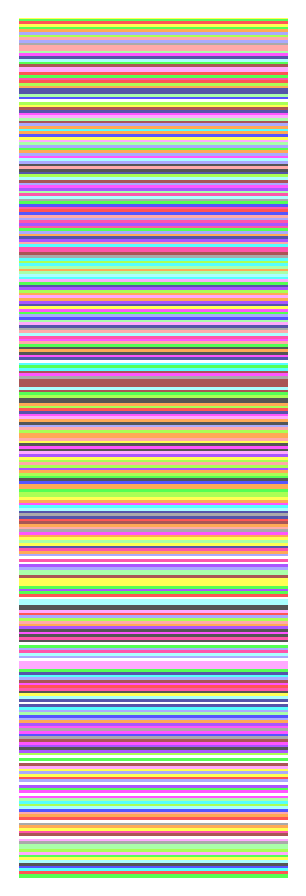
\includegraphics[width=0.14\textwidth]{resource/ground_truth.eps}
    }
    \subfigure[Random Noise]{
    \label{subfig:er_pdf}
    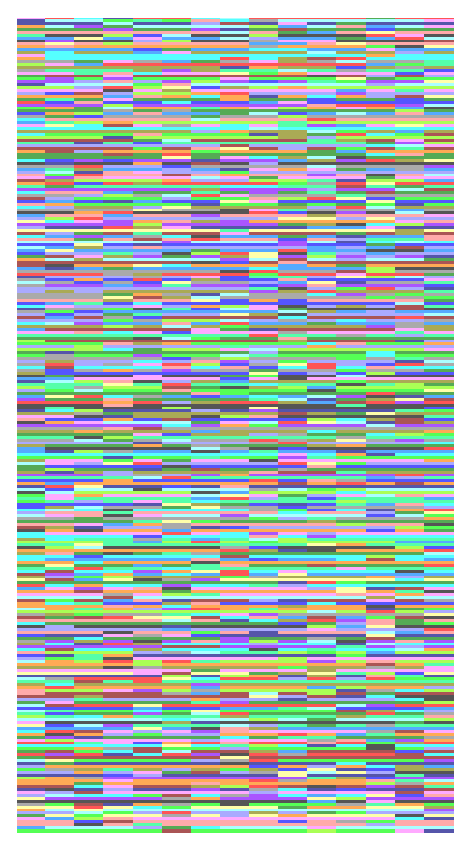
\includegraphics[width=0.14\textwidth]{resource/random_error.eps}
    }
    \subfigure[Outlier Reject]{
    \label{subfig:re_pdf}
    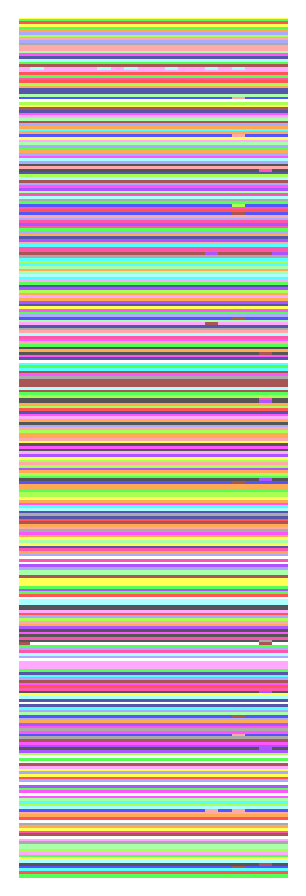
\includegraphics[width=0.14\textwidth]{resource/recover.eps}
    }
    \caption{visualized results of the synthetic dataset} \label{fig:ensemble_cluster}
\end{figure}


\subsection{Feature Extraction}
In this section, we describe the details of the feature extraction for each dataset. 
All convolutional neural network(CNN) features are extracted using Caffe~\cite{jia2014caffe}, a deep learning framework.

In UCF101 dataset, five different features are extracted from the following:
\begin{itemize}
  \item `fc6' of C3D~\cite{tran2015learning}
  \item `pool5/7x7\_s1' from GoogleNet~\cite{szegedy2015going}
  \item `pool5' of ResNet-152~\cite{he2015deep}
  \item two `fc6's of Two-Stream~\cite{simonyan2014two}
\end{itemize}
Given a video, we extract the above five features following the same process in~\cite{simonyan2014two,tran2015learning}(GoogleNet and ResNet-152 feature are same as spatial net in~\cite{simonyan2014two}). 
All models we used are available on Internet provided by authors.

In Cifar10 dataset, the features are extracted from the `global\_pool' layer of ResNet-20,32,44,56,68,110~\cite{he2015deep} and of pre-activation ResNet-20,32,44,56,68,110,164 models~\cite{he2016identity}. 
Another feature is extracted from `pool3' layer's features of cifar10\_full model described in caffe example prototxt\footnote{\url{https://github.com/BVLC/caffe/blob/master/examples/cifar10/cifar10_full.prototxt}}. 
We train each ResNet model following the standard procedure in~\cite{he2015deep,he2016identity} and cifar10\_full model using a official shell\footnote{\url{https://github.com/BVLC/caffe/blob/master/examples/cifar10/train_full.sh}} before extracting features. 
In Cifar100 dataset, we use the same model and process as in Cifar10 except the caffe example model and pre-activation ResNet-68, totaly twelve features.

In all other experiments, eight different features are extracted from the following:
\begin{itemize}
  \item `fc6' of VGG16,VGG19~\cite{chatfield2014return}
  \item `fc6' of AlexNet,CaffeNet~\cite{krizhevsky2012imagenet}
  \item `pool5/7x7\_s1' from GoogleNet~\cite{szegedy2015going}
  \item `pool5' of ResNet-50,101,152~\cite{he2015deep}
\end{itemize}
We use the offical caffe model provided by Caffe Model Zoo\footnote{\url{https://github.com/BVLC/caffe/wiki/Model-Zoo}}.
For above eight features, we don't do extra operation.


\subsection{Experiment on UCF 101 dataset}

For action recognition, we present our results on UCF 101 dataset~\cite{soomro2012ucf101}. 
UCF101 contains 13320 videos collected from YouTube, categoried into 101 human action classes. 
We use the official split1 described in~\cite{soomro2012ucf101}, which have 9573 training videos and 3783 testing videos. 

As mentioned above, we extract fives features and train different classifier on each feature with the default parameters by liblinear. 
Appling five classifiers on test data, we obtain 5 * 101 confidence scores for each video, which forms the input matrix X of our algorithm. 
Results are shown in Table~\ref{table:ucf101}, in which we illustrate the performance of the best single classifier and compare six fusion methods. 
To be noted, FWOT~\cite{xuiccv2013feature} is too slow to train, we didn't show it's result (more than one day).

\begin{table}[h]\small
\centering
\label{table:ucf101}
\begin{tabular}{c|c}
\hline
Method                       & Mean Accuracy(\%) \\\hline
SVM on Temporal Net Features & 86.23\%           \\\hline
ASF                          & 86.78\%           \\
MKL                          & 85.38\%           \\
RCEC                         & 86.60\%           \\          %ori: 0.88290  vote : 0.88158
FWOT                         & -                 \\
LPBoost                      & 86.24\%           \\\hline
Ours                         & 89.03\%           \\          %ori: 0.8888   vote : 0.88686
\hline
\end{tabular}
%\caption{Mean Accuracy on UCF101 dataset for best single model and six fusion methods}
\caption{Mean Accuracy on UCF101 dataset}
\end{table}


\subsection{Experiment on Cifar10 dataset}

In CIFAR-10 dataset~\cite{krizhevsky2009learning}, totally 60000 32x32 colour pictures are categoried into 10 classes, with 6000 pictures per class. 
There are 50000 training data and 10000 testing data. 
Fourteen CNN features are extracted from multiple state of the art models. 
This experiments show the ability of our algorithm to handle large scale data.

As we have 50000 training data and 10000 testing data, FWOT~\cite{xuiccv2013feature} has one step to deal with N*N matrixes, which are excessive to train~(more than one day). 
LPBoost~\cite{gehler2009feature} need to create a $NK\times N$ constraint matrix linear programming solvers\footnote{The author use the MOSEK interior-point solver, see www.mosek.com.}, which occupies too much memory and still consumes long time to train, so we solve this problem by using sparse matrix storage and parallel during matlab. 
We also use `-s 2' parameters in liblinear to speedup training process. Results of other contrast algorithms are shown on \ref{table:cifar10}


\begin{table}[h]\scriptsize
\centering
\label{table:cifar10}
\begin{tabular}{c|c|c}
\hline
Method  & Mean Accuracy     & Classification Time + Fusion Time(s)\\\hline
ASF     & 94.21\%           & 55.6 + 0.02                         \\
MKL     & 94.15\%           & 865.09                              \\
RCEC    & 94.99\%           & 55.6 + 3.5                          \\         % ori:0.94850  vote:0.94820 / 0.95070
FWOT    & -                 & -                                   \\
LPBoost & 94.88\%           & 54.99                               \\\hline
Ours    & 95.11\%           & 55.6 + 32.1                         \\         % ori:0.95050  vote:0.95030
\hline
\end{tabular}
\caption{Mean Accuracy and Time cost on cifar10 dataset}
\end{table}

\subsection{Experiment on Cifar100 dataset}

CIFAR-100~\cite{krizhevsky2009learning} is similar with CIFAR-10, except it has 100 classes containing 600 images each.
There are 50000 training data and 10000 testing data as CIFAR-10. 
Twelve CNN features used in this experiment are described in the previous section. 
Training and comparison process are the same as CIFAR-10. Results are shown as below:


\begin{table}[h]\small
\centering
\label{table:cifar100}
\begin{tabular}{c|c}
\hline
Method  & Mean Accuracy \\\hline
ASF     & 76.91\%           \\
MKL     & 72.71\%           \\
RCEC    & 77.13\%           \\  %ori: 0.76960,  vote: 0.77050
FWOT    & -                 \\
LPBoost & 76.59\%           \\\hline
Ours    & 77.72\%           \\  %ori: 0.77170, vote: 0.77160
\hline
\end{tabular}
\caption{Mean Accuracy on cifar100 dataset}
\end{table} 

\subsection{Experiment on Oxford-IIIT-Pet dataset}

The Oxford-IIIT-Pet dataset~\cite{parkhi12a} contains 7349 images covering 37 different breeds of cats and dogs, 2371 images for cats and 4978 images for dogs. 
Each categories have about 200 pictures with a large variations in multiple views, such as scale, pose and lighting.
We randomly sample fifty percent pictures as our training data and the others as our testing data, repeat ten times. We first traing svm on each seperate features and fuse by our ORLF method. The comparison results are shown as below:

\begin{table}[h]\small
\centering
\label{table:oxford_pet}
\begin{tabular}{c|c}
\hline
Method                       & Mean Accuracy     \\\hline
ASF                          & 92.46\%           \\
MKL                          & 87.13\%           \\
RCEC                         & 92.11\%           \\          % ori: 92.41
FWOT                         & 92.90\%           \\			 
LPBoost                      & 92.73\%           \\\hline
Ours                         & 92.90\%           \\			 % ori: 92.84
\hline
\end{tabular}
\caption{Mean Accuracy on Oxford-IIIT-Pet dataset}
\end{table}



\subsection{Post Strategy Selection}
In this section, we first compare three proposed final post strategy on three small dataset: PASCAL VOC 2007~\cite{pascal-voc-2007}, Oxford Flowers 17~\cite{nilsback2006visual} and Caltech 101~\cite{Li2006One}.
PASCAL VOC 2007 contrains 6146 images classified into 20 classes, after filtering the multi-label data. 
Oxford Flowers 17 dataset havs 17 flower categories with 80 images for each class. 
Caltech 101 contains a total of 9,146 images, split between 101 distinct object categories and a background category.
We sample fifty percent data as training data and the others as testing data, repeat 10 times on all three datasets.

Experiment results show that the first strategy outperforms than the others in most cases and never performes under the others. 
The reason that the first strategy is better than the second one might because the soft average method would reserve more detail information than the hard voting method.
Since the recover matrix X contains the outlier rejection information, 
the last strategy combines the outlier results as a rejection decision operating on the original confidence score matrix, which utlizing more than both the first and second strategy.

\begin{table}[h]\small
\centering
\label{table:strategy}
\begin{tabular}{c|c|c|c}
\hline
Method                       & VOC 2007 &  Flowers 17  & Caltech 101 \\\hline
Strategy 1                   & 89.60\%  &  96.77\%     &   96.04\%   \\\hline
Strategy 2                   & 89.41\%  &  96.61\%     &   95.91\%   \\\hline
Strategy 3                   & 90.10\%  &  96.77\%     &   96.08\%   \\
\hline
\end{tabular}
\caption{Mean Accuracy on Three Strategies}
\end{table}


\subsection{\yanred{Unwork dataset Record Data}}

\yanred{On PASCAL VOC 2007 and Oxford Flowers 17 Datasets.}

\begin{table}[h]\small
\centering
\label{table:voc2007}
\begin{tabular}{c|c}
\hline
Method                       & Mean Accuracy     \\\hline
ASF                          & 89.04\%           \\
MKL                          & 85.53\%           \\
RCEC                         & 89.60\%           \\
FWOT                         & 89.85\%           \\
LPBoost                      & 90.54\%           \\\hline
Ours                         & 90.10\%           \\
\hline
\end{tabular}
\caption{VOC 2007}
\end{table}


\begin{table}[h]\small
\centering
\label{table:flower17}
\begin{tabular}{c|c}
\hline
Method & Mean Accuracy\\\hline
ASF    &  96.81\% \\
MKL    &  93.24\% \\
RCEC   &  96.81\% \\
FWOT   &  96.88\% \\
LPBoost & 97.24\% \\\hline
Ours   &  96.74\% \\
\hline
\end{tabular}
\caption{Oxford Flowers 17}
\end{table}


\iffalse
\subsection{Experiment on PASCAL VOC 2007 dataset}
PASCAL VOC 2007 is a dataset for object detection and image classification. For our experiment we only use the image level annotation information. Since each image may contain more than one label, we filter the multilabel images. Using the offical split provided by \cite{pascal-voc-2007}, we have 2954 trainval images and 3192 test images with 20 classes after filtration. We extract features from AlexNet,VGG,GoogleNet,ResNet, totally seven diffierent CNN features(AlexNet for alexnet and caffenet, VGG for VGG16 and VGG19, ResNet for ResNet50 and ResNet101).

After the procesure of classification and fusion, we got the results as \ref{table:voc}. Since in PASCAL VOC 2007 dataset, more classifiers are utilized than UCF101, it's clear that our method achieve significant improvement than single model and a slight improvement than other fusion algorithm.

\subsection{Experiment on Oxford Flowers}
Oxford Flowers 17 dataset~\cite{nilsback2006visual} havs 17 flower categories with 80 images for each class. There are three predefined splits training set with 680 images, validation set with 340 images and testing set 340 images. 2048 dimetions `pool5' features from ResNet-50,101,152 proposed in \cite{he2015deep} and 4096 dimetions `fc6' features from CaffeNet,AlexNet proposed in \cite{krizhevsky2012imagenet} are used for linear SVM. The models are download from Caffe Model Zoo\footnote{\url{https://github.com/BVLC/caffe/wiki/Model-Zoo}}, with no finetuning on the current dataset.

We use the predefined training set and validation set as our training data, trained on liblinear with default parameters. For LPBoost Methods, we use 5 fold cross validation to select the best hyperparmeter $\nu$.
Results are shown in \ref{table:flower17}

\fi


\begin{quote}
\begin{small}
  \bibliographystyle{aaai}
  \bibliography{ensemble_clustering}
\end{small}
\end{quote}

\end{document}
